\documentclass[a4paper,10pt,titlepage]{report}

\usepackage[utf8]{inputenc}
\usepackage[T1]{fontenc}
\usepackage{textcomp}
\usepackage[usenames,dvipsnames]{xcolor}

\usepackage{listings}
\definecolor{lbcolor}{rgb}{0.95,0.95,0.95} 
\lstdefinestyle{base}{
  language=C,
  emptylines=1,
  breaklines=true,
  basicstyle=\ttfamily\color{black},
  moredelim=**[is][\color{violet}]{@*v}{@*v},
  moredelim=**[is][\color{ForestGreen}]{@*f}{@*f},
  moredelim=**[is][\color{red}]{@*r}{@*r},
  moredelim=**[is][\color{blue}]{@*b}{@*b},
  showstringspaces=false
}
\lstset{
    frame=no,
    xleftmargin=\fboxsep,
    xrightmargin=-\fboxsep, 
    backgroundcolor=\color{lbcolor},
    style=base
}

\usepackage{graphicx}
\usepackage{epstopdf}
\usepackage{url}

%Non sillabare
\tolerance=1
\emergencystretch=\maxdimen
\hyphenpenalty=10000
\hbadness=10000

\lstset{columns=fullflexible,basicstyle=\ttfamily}
\usepackage{graphicx}

\title{MetaC}
\author{Daco Harkes, Ioana Jivet, Dario Nesi, Mircea Voda}
\date{Spring 2013}

\begin{document}
\begin{titlepage}
\begin{center}


% Upper part of the page. The '~' is needed because \\
% only works if a paragraph has started.

\includegraphics[width=0.25\textwidth]{pics/logo.eps}~\\[1cm]

\textsc{\LARGE Delft University of Technology}\\[4.5cm]

\textsc{\Large Model-Driven Software Development}\\[1cm]

% Title
{ \Huge \bfseries{MetaC}\\[1.5cm]}

\emph{Spring 2013}\\[4cm]

% Author and supervisor
\begin{minipage}{0.4\textwidth}
\begin{flushleft} \large
\emph{Students:}\\
Daco \textsc{Harkes}\\
Ioana \textsc{Jivet}\\
Dario \textsc{Nesi}\\
Mircea \textsc{Voda}\\
\end{flushleft}
\end{minipage}
\begin{minipage}{0.4\textwidth}
\begin{flushright} \large
\emph{Professor:} \\
Dr. Eelco \textsc{Visser}
\end{flushright}
\end{minipage}

\vfill

\end{center}
\end{titlepage}



\chapter{Introduction}

While the C programming language provides good support for writing efficient, low-level code, it is not adequate for defining higher-level abstractions relevant to embedded software. This project addresses that problem and proposes a language inspired by mbeddr \cite{voelter2012mbeddr} that provides object-oriented functionalities to embedded software developers. The main advantage of MetaC over mbeddr is that MetaC is a textual language rather than a projectional language.

MetaC results so a domain specific language oriented to the development of reliable and highly maintainable software, equipped with extensions such as State Machine Modelling and Runtime Message Reporting that exempts programmers from writing boilerplate code.

The language has been built on the solid basis of BaseC, that is described in detail in this document, and implemented via Stratego/XT \cite{visser2004program} and Spoofax \cite{kalleberg2007spoofax} technologies. 

Issues as architecture-independence and extensibility have been tackled in the Spring of 2013 at the TU Delft University, during the course of Model-Driven Software Development, by four students leaded by Professor Eelco Visser and supported by the Software Engineering Research Group for one semester.

This documentent is structured as follows. In the next section, a Conceptual view of mbeddr is given, with references to this project, in order to evidence strengths of both solution. In section 3, BaseC implementation details are described, with a description of the standard development process used to obtain executable software starting from MetaC programs, and focusing on aspects of syntax and name binding. Sections 4 and 5 contain two DSLs for State Machines Modelling and Runtime Message Reporting , along with implementation and usage aspects. The last section describes future improvements. The appendices contain a quick reference is provided to be used as handy manual.

\chapter{Concepts of MetaC}

MetaC is inspired by mbeddr. mbeddr is a language that provides support for developing embedded software. The main difference between mbeddr and MetaC is that mbeddr uses a projectional editor while MetaC is a textual language.

mbeddr enables C programmers to use abstract concepts that are not allowed in standard C as State-Machine-based reasoning or object-oriented modularity. Those concepts can be heavily used for tailoring software to the embedded domain to produce software more maintainable and fixable. Moreover, features that are prohibited in the majority of standards have been removed, in order to keep the software stable and reliable.

mbeddr has been designed with MPS \cite{voelter2010language}. Its approach is radically different from the other embedded development tools, third parties can use the same mechanisms for building their own extensions that were used to implement C and the existing extensions. MPS has a projectional editor, directly manipulating the AST instead of parsing text, which makes building extensions to the syntax easier. 

Also, mbeddr embody tools to support key aspects of the Software Engineering Process as Requirement Verification and Documentation. Via MPS it provides functionalities as such as Model Checking and Contract verification.

MetaC is a textual language instead of being a projectional language. The main advantage of this is to not need any specific environment to be used in its core functionality and to be able to use plaintext based tools such as version control with the source code. 

MetaC provides support to a big variety of data type that are platform independent, as mbeddr, but also allows old-style C constructs that experienced programmers can exploit to produce very efficient code.

Also, object-oriented reasoning is enabled by the mbeddr-like concept of module and this way C is enriched by features as encapsulation and inheritance that programmers can use in code in an elegant fashion.

The State Machine Modelling and Runtime Message Reporting extensions are ported from mbeddr. This way the effort for code migration from mbeddr and maintainability are minimized. Software writtin in mbeddr can be easily ported to MetaC, if the all extensions used in mbeddr are available.


\chapter{BaseC}

BaseC is a language based on C but abstracting over tradtional .c and .h files. 
MetaC is BaseC plus extensions, and will be covered in the next chapters. In this chapter BaseC is described in detail. 

\section{Syntax}

The top level concept in MetaC programs are modules. Modules act as namespaces and as the unit of encapsulation. The classical separation between .c and .h files doesn’t exists in MetaC. The code resides in .mc files that get transformed to .c and .h files during the generation phase. 
A module can import other modules. The importing module can then access the exported contents of imported modules. Module contents can be exported using the keyword exported. All other syntax is simply C.

A basic module is shown in code snippet below.

\begin{lstlisting}
module HelloWorld {
    int32 main() {
        return 0;
    }
}
\end{lstlisting}



\section{Name binding and type checking}
The namebinding for BaseC follows the same rules as basic C. However, the scope of entities declared inside modules without the “exported” specifier is limited and these entities are not visible outside the module.

Unlike usual C IDEs, MetaC provides \textbf{type checking} during editing, and not only after an explicit compilation. The type checking is performed on statements, expressions and declarations with initialization, that include variables, numerals and function calls. Additionally, the return types and parameter types of function calls are also type checked.

Like in C, \textbf{typedefs} define synonym types to already existing types. In MetaC, when the type checking encounters a synonym type, it recursively extracts the base type, which is then used in the type checking.
 

\section{Mapping to C and Building}

\begin{figure}[ht!]
\centering
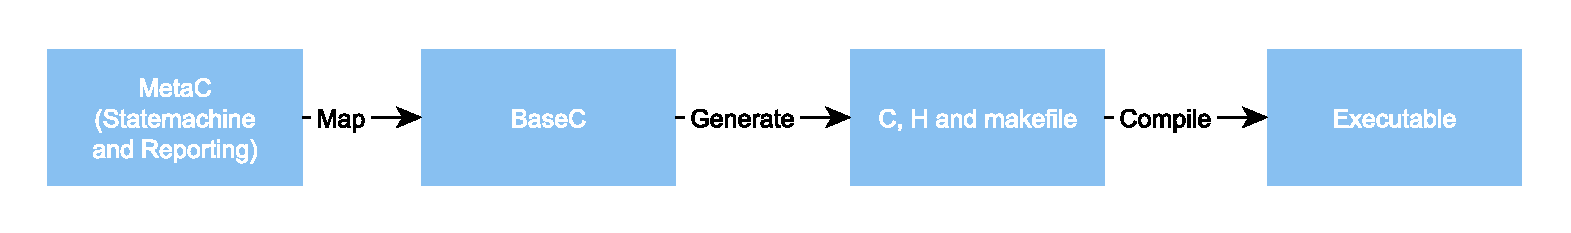
\includegraphics[width=\linewidth]{pics/compilation_simple.eps}
\caption{The transformation steps in compilation of MetaC}
\label{fig:compilation_simple}
\end{figure}

In the bigger picture the mapping from BaseC to C is called the generate step as is shown in Figure ~\ref{fig:compilation_simple}. MetaC is mapped to c and h files together with a make file. Every module generates one c file and one header file. External modules only generate a header file (see next subsection for that). This mapping is based on the way mbeddr maps its modules to c, h and makefile.

{\setlength{\parindent}{0cm}

The c corresponding to a MetaC module contains:
\begin{itemize}
\item Its corresponding header file
\item The header files of the imported modules
\item Declarations
\item Function definitions
\item Structs, Unions and Enums
\end{itemize}


The accompanying header file contains:
\begin{itemize}
\item standard ifndef define
\item all external functions
\end{itemize}

The makefile contains:
\begin{itemize}
\item All object file targets for all modules
\end{itemize}
}
For multiple files the imports are chased iteratively as is shown in Figure ~\ref{fig:trace_imports}. A check is done to ensure modules referenced more than once is only included once in this process. Cyclic references are solved the same way.

\begin{figure}
\centering
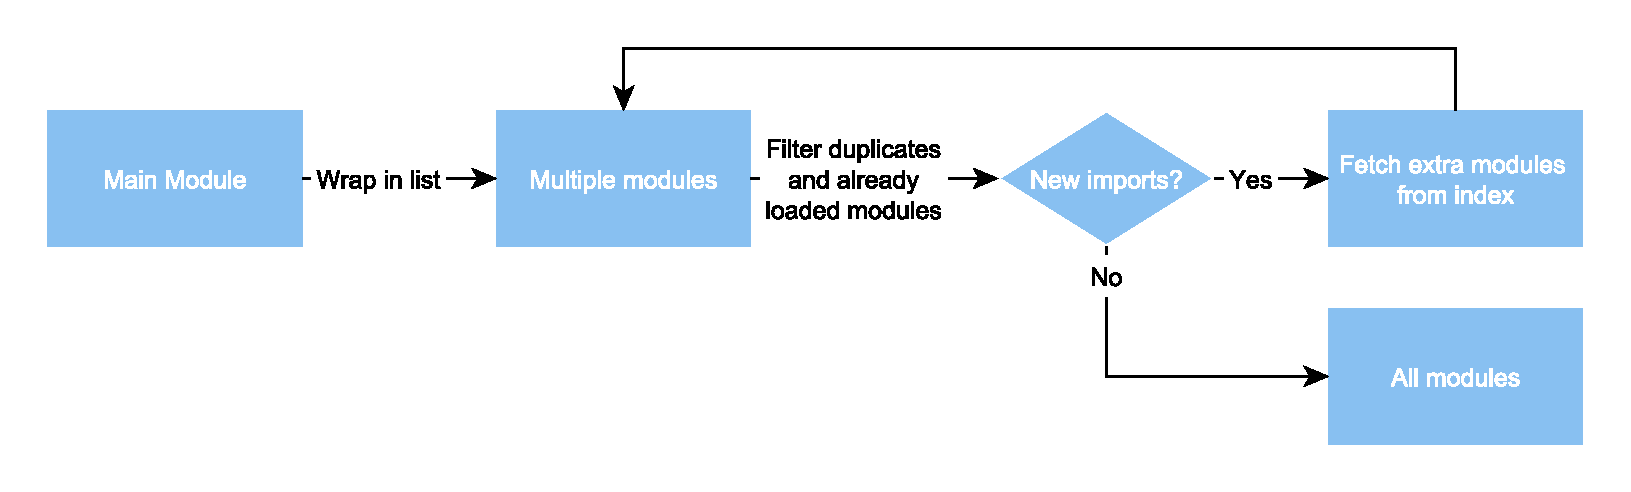
\includegraphics[width=\linewidth]{pics/tracing_imports.eps}
\caption{Tracing imports}
\label{fig:trace_imports}
\end{figure}

After the c files, the headers files and the makefile are generated make with gcc is called, which compiles the program into an executable. This can bee seen in Figure ~\ref{fig:compilation_complete} which also shows the last part of the complete build process.

\begin{figure}[ht!]
\centering
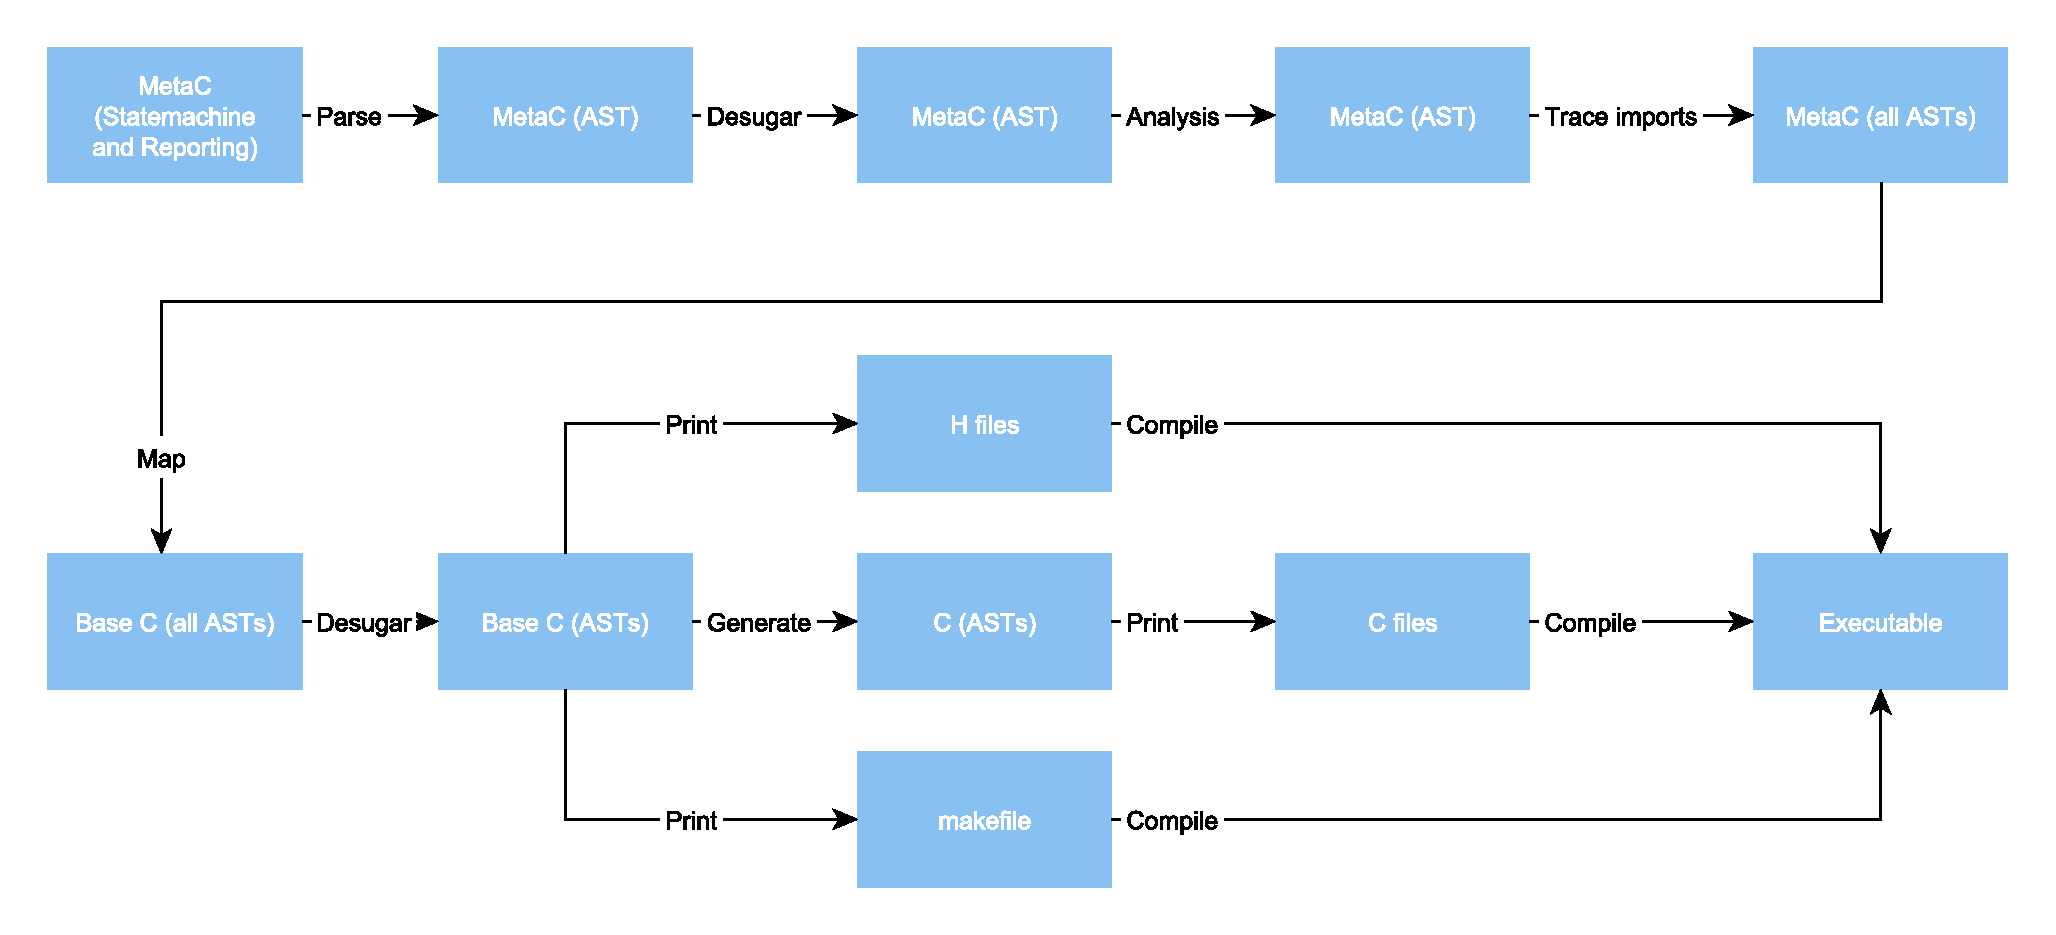
\includegraphics[width=\linewidth]{pics/compilation_complete.eps}
\caption{The complete build process of MetaC}
\label{fig:compilation_complete}
\end{figure}

\subsection{Example program with two modules}
Here we show an example with two modules. The MetaC files (*.mc) show the source code, and the other files the generated c, h and make-file(s) which are fed to gcc.\\

{\setlength{\parindent}{0cm}

test52.mc
\begin{lstlisting}
module test52 imports factorial{
    exported int32 main(int32 argc, string[] argv) {
        printf("5! is %d \n", fact(5));
        return 0;
    }
}
\end{lstlisting}

factorial.mc
\begin{lstlisting}
module factorial{
    exported int32 fact(int32 x){
        if (x <= 1)
            return 1;
        return x * fact(x-1);
   	}
    
}
\end{lstlisting}

test52.h
\begin{lstlisting}
#ifndef TEST52
#define TEST52
 
#include <stdint.h>
 
int32_t main (int32_t argc, int8_t * argv []);
 
#endif
\end{lstlisting}

test52.c
\begin{lstlisting}
#include "test52.h"
#include <stdlib.h>
#include "factorial.h"
int32_t main (int32_t argc, int8_t * argv [])
{
    printf("5! is %d \n", fact(5));
    return(0);
}
\end{lstlisting}

factorial.h
\begin{lstlisting}
#ifndef FACTORIAL
#define FACTORIAL
 
#include <stdint.h>
 
int32_t fact (int32_t x);
 
#endif
\end{lstlisting}

factorial.c
\begin{lstlisting}
#include "factorial.h"
#include <stdlib.h>
int32_t fact (int32_t x)
{
    if((x <= 1))
        return(1);
    return((x * fact((x - 1))));
}
\end{lstlisting}

makefile
\begin{lstlisting}
CC=gcc
CFLAGS=-std=c99
ODIR=./bin
_OBJ_test52=test52.o factorial.o
OBJ_test52=$(patsubst %,$(ODIR)/%,$(_OBJ_test52))
 
 
all: removeStuffFromLibraries clean test52
.PHONY: removeStuffFromLibraries all clean
removeStuffFromLibraries:
   	
$(ODIR)/%.o: %.c
         	mkdir -p $(ODIR)
   	$(CC) $(CFLAGS)   -c -o $@ $< 
debug: CFLAGS +=-g
debug: clean test52
test52: $(OBJ_test52)
   	$(CC) $(CFLAGS) -o $@ $^  
clean:
   	rm -rf $(ODIR) 
\end{lstlisting}

}

Note that all header files include \emph{stdint.h} and that all .c files include \emph{stdlib.h} because these are needed for the test programs without external modules. In the future these should be removed.

\section{External: standard C libraries}
Standard C libraries can be included by using external modules. These external resources can be imported by using the resource keyword. External modules are not compiled themselves, only the libraries they reference are imported. The remainder of this section contains one example with the resulting c code showing how this works in practise.

{\setlength{\parindent}{0cm}

test50.mc
\begin{lstlisting}
module test50 imports c_stdio{
    exported int32 main(int32 argc, string[] argv){
        int32 a = 3;
        printf("%d",a);
        return 0;
    }
}
\end{lstlisting}

c\_stdio.mc
\begin{lstlisting}
external module c_stdio resources stdio.h {
    void printf(string formatString, int32 arg1);
}
\end{lstlisting}

test50.h
\begin{lstlisting}
#ifndef TEST50
#define TEST50
#include <stdint.h>
int32_t main (int32_t argc, int8_t * argv []);
#endif
\end{lstlisting}

test50.c
\begin{lstlisting}
#include "test50.h"
#include <stdlib.h>
#include "c_stdio.h"
int32_t main (int32_t argc, int8_t * argv [])
{
    int32_t a = 3;
    printf("%d", a);
    return(0);
}
\end{lstlisting}

c\_stdio.h
\begin{lstlisting}
#include <stdio.h>
\end{lstlisting}

makefile
\begin{lstlisting}
CC=gcc
CFLAGS=-std=c99
ODIR=./bin
_OBJ_test50=test50.o
OBJ_test50=$(patsubst %,$(ODIR)/%,$(_OBJ_test50))
 
all: removeStuffFromLibraries clean test50
.PHONY: removeStuffFromLibraries all clean
removeStuffFromLibraries:
  	
$(ODIR)/%.o: %.c
        	mkdir -p $(ODIR)
  	$(CC) $(CFLAGS)   -c -o $@ $< 
debug: CFLAGS +=-g
debug: clean test50
test50: $(OBJ_test50)
  	$(CC) $(CFLAGS) -o $@ $^  
clean:
  	rm -rf $(ODIR) 
\end{lstlisting}

}

\chapter{Reporting DSL}
The implementation of the reporting DSL is relatively straightforward. The message constructor has the form \emph{Message(id, paramList, modifier, messageText)} where messageText is a string representing the contents of the message. 

The example below shows the parsing of a message declaration.

\begin{lstlisting}
INFO HelloWorld() active: "Hello, World!"
\end{lstlisting}

\begin{lstlisting}
Message(
    Identifier("HelloWorld"), 
    [], 
    MessageActive(), 
    String("\"Hello, World!\"")
)
\end{lstlisting}

During indexing, the last term of the constructor (the message text) is stored in the index as \textbf{MsgText()} data. This term (messageText) is later retrieved from the index during the to-basec phase (see the complete build process of MetaC) in order to translate \textbf{Report} statements into \textbf{printf()} function calls. The messageText is used as the parameter for the \textbf{printf()} call.

\section{Example}
\begin{lstlisting}
module HelloWorld { 
    exported int32 main(int32 argc, string[] argv) { 
        report m.HelloWorld(); 
        return 0;
    }
    messagelist m { 
        INFO HelloWorld() active: "Hello, World!"
    }
}
\end{lstlisting}

\newpage
{\setlength{\parindent}{0cm}
The report statement: 
}
\begin{lstlisting}
report m.HelloWorld(); 
\end{lstlisting}
{\setlength{\parindent}{0cm}
will be translated to:
}
\begin{lstlisting}
printf("Hello, World!");
\end{lstlisting}


\chapter{State Machine DSL}

The State Machine DSL is the main C extension implemented for MetaC. This extension allows the definition and usage of State Machines inside regular MetaC code. The MetaC State Machine DSL closely follows the mbeddr implementation of State Machines.

\section{Syntax}
The syntax for the State Machine DSL follows the one used by mbeddr and can be divided into State Machine definition syntax and State Machine operation in BaseC syntax.
\subsection{Definition}
A State Machine is defined by using the following construction. The State Machine name has to be a valid identifier according to BaseC, and the initial state must be defined as a state inside the State Machine.

\begin{lstlisting}
statemachine statemachine_name initial = initial_state.
\end{lstlisting}

{\setlength{\parindent}{0cm}
A State Machine has several components:
}
\begin{itemize}
\item \emph{inner variables}, declared using the keyword \textbf{var};
\item \emph{State Machine states}, declared using the keyword \textbf{state};
\item \emph{transition triggering events}, declared using the keyword \textbf{in};
\item \emph{outer events}, declared using the keyword \textbf{out};
\end{itemize}
 
In and out events must be declared before they can be used in states to describe transitions. Their declaration is the same as for function prototypes, except for the missing return type. In addition, the out events have to be bound to an external function, called when the outer events are triggered.

\begin{lstlisting}
state beforeFlight {
    entry { points = 0; }
    on next [tp->alt > 0] -> airborne
    on report[]-> beforeFlight {printf("STATE: beforeFlight");}
    exit { points += TAKEOFF; }
}
\end{lstlisting}

{\setlength{\parindent}{0cm}
State machine states have three elements, all of them optional.
}
\begin{itemize}
\item \emph{entry} clause defines a block of instructions executed when entering the state;
\item \emph{exit} clause defines a block of instructions executed before leaving the state;
\item transitions, marked by the keyword on. In the general syntax for transitions, the transition condition is expressed between square brackets as a boolean expression, with the parameters of the transition triggering event, declared at the State Machine level. The instructions that need to be executed during the transition are listed in an optional block.
\end{itemize}
 
\begin{lstlisting}
on <trigger_event> [ <condition> ] -> <target_state> <block?>
\end{lstlisting}

\subsection{Integration with BaseC}
In BaseC, State Machines are defined inside modules, next to structs and functions. Similarly to structs, a State Machine definition generates a new type. Further, one can declare variables that have State Machine types previously defined.

\begin{lstlisting}
module AnalyzeFlight{
    statemachine analyzeFlight initial = beforeFlight {
        ...
    }
    exported int8 main(int32 argc, string[] argv) {	  
        statemachine analyzeFlight smvar;
        return 0;
    }	
}
\end{lstlisting}

Handling State Machine variables is done through three predefined functions: two translate into BaseC statements (sminit and smtrigger), and one into a BaseC expression (smIsInState).

\begin{itemize}
\item \textbf{sminit(smvar);} initializes the internal variables of the State Machine and sets the initial state. The only parameter points to a variable of a State Machine type.

\item \textbf{smtrigger(smvar, report());} sends an event to the State Machine. The two parameters point to the State Machine variable and the in event that needs to be analyzed.

\item \textbf{smIsInState(smvar, statename);} checks whether the State Machine’s current state is the one indicated by the second parameter. The \emph{statename} parameter is an identifier describing an existing state of the State Machine.
\end{itemize}

\section{Type checking and name binding}
Since the State Machine DSL is built upon BaseC, most of the typechecking and name binding are inherited from BaseC. The additional name binding is related to states, events, inner variables and outer events to functions defined in BaseC. 

In the State Machine definition, no additional type checking is needed, other than the one inherited from BaseC. However, type checking rules are necessary when the State Machine DSL is integrated into BaseC. A State Machine definition generates a type, so it has to be integrated in the type system, similarly to structs. Further type checking is done on the call parameters of the predefined functions for State Machine handling.

\section{Mapping to BaseC}

The State Machine to BaseC mapping transforms the State Machine constructor into a list consisting of headerAST, initFunction and executeFunction. 

The \textbf{headerAST} contains:
\begin{itemize}
\item an enum that is used to store the states of the State Machine 
\item an enum used to store the events that the State Machine can react to
\item a struct that contains internal variables defined by the State Machine + a special field (\_\_currentState) that is used to store the current state of the State Machine
\end{itemize}

The \textbf{initFunction} has the role of initializing the variables of the State Machine and the \_\_currentState variable to their default values. The function has one parameter: a pointer to the State Machine variable that needs to be (re-)initialized.

The \textbf{executeFunction} is the ‘engine’ of the State Machine. It has 3 parameters:  a pointer to the State Machine variable, the name of the event and a (double) pointer to a void variable that is used to pass the event arguments to the State Machine.
The executeFunction is structured as nested switch-case statements.
The outer switch statement checks the current state of the State Machine. Each case statement matches a particular state and has as a ‘body’ another switch statement that checks the current event. The case statements of the event switch match only the events  that can be received in that state and the body of these event case statements consists of the statements contained in the entry, exit and transition blocks of the state. First, the statements from the current state’s exit block are generated, followed by the statements from the appropriate transition block, a statement that changes the value of the current state variable to the corresponding next state and finally, the statements found in the next state’s entry block. 
The transition from one state to another can also be controlled with a boolean condition. If this is the case, the statement described above are generated inside an if statement block which checks that condition.

\newpage

\subsection{Example}
{\setlength{\parindent}{0cm}
State Machine definition
}

\begin{lstlisting}
statemachine counter initial = start { 
    readable var int8 current = 0
    in increment(int8 delta)  
    in reset()
    state start { 
        entry { 
            @*fcurrent = 0;@*f  
        } 
        exit {
            @*bprintf("exit start\n");@*b
        }  
        on increment[@*rdelta<15@*r]-> 
            increasing {@*vcurrent +=delta;@*v}
    }
	  
    state increasing {
        entry{
            printf("in increasing: current: %d\n",current);
        }
        on reset[] -> start {printf("statemachine reset\n");}
        on increment[delta<5 && current<5]-> increasing {current +=delta;}
    } 
}
\end{lstlisting}
{\setlength{\parindent}{0cm}
headerAST
}
\begin{lstlisting}
enum moduleName_sm_events_counter{
    counter__event_increment,
    counter__event_reset 
};
enum moduleName_sm_states_counter{
    counter__state_start,
    counter__state_increasing 
};
struct moduleName_sm_data_counter{
    enum moduleName_sm_states_counter __currentState;
    int8_t current;
};
\end{lstlisting}   
{\setlength{\parindent}{0cm}
initFunction
}
\begin{lstlisting}
void moduleName_sm_init_counter(
    struct moduleName_sm_data_counter * instance){

    instance->__currentState = counter__state_start;
    instance->current = 0;
}
\end{lstlisting}    
\newpage
{\setlength{\parindent}{0cm}
executeFunction
}
\begin{lstlisting}
void moduleName_sm_execute_counter(
    struct moduleName_sm_data_counter* instance, 
    enum moduleName_sm_events_counter event, 
    void** arguments){
    switch ( instance->__currentState ){
        case counter__state_start:{
            switch(event){
                case counter__event_increment:
                {
                    @*rif((((*((int8_t*)arguments[0])))<15))@*r
                    {
                        @*bprintf("exit start\n");@*b
                        @*vinstance->current += 
                            ((*((int8_t*)arguments[0])));@*v
                        instance->__currentState = 
                            counter__state_increasing;
                        printf("in increasing: current: %d\n", 
                            instance->current);
                        return(-1);
                    }break;
                }
            }break;
        }
        case counter__state_increasing:{    
            switch(event){
                case counter__event_reset:{
                    {
                        printf("statemachine reset\n");
                        instance->__currentState = 
                            counter__state_start;
                        @*finstance->current = 0;@*f
                        return(-1);
                    }break;
                }
                case counter__event_increment:{
                    if(((((*((int8_t*)arguments[0]))) < 5) && 
                        (instance->current < 5)))
                    {
                        instance->current +=
                            ((*((int8_t*)arguments[0])));
                        instance->__currentState = 
                            counter__state_increasing;
                        printf("in increasing: current: %d\n",
                            instance->current);
                        return(-1);
                    }break ;
                }
            }break;   }}}
\end{lstlisting}

\chapter{Future work}
MetaC is a solid base for future expansions. The language provides basic functionality with modules and has the reporting and State Machine DSLs. Some suggested features can be found on the issue tracker of MetaC \footnote{\url{http://yellowgrass.org/project/MetaC}}.

\section{Import all std. C libraries automatically}
One suggestion to improve MetaC is to automatically generate all external modules wrapping C standard libraries. The glibc is however full of macros, which make it non trivial to extract the external function definitions. Discussing this feature can be done on the issue tracker \footnote{\url{http://yellowgrass.org/issue/MetaC/39}}.

\section{Import custom C libraries}
An important feature for MetaC is the use of external custom C libraries. This is important as developers can keep using existing systems and build MetaC on top of these systems. As with the standard C libraries this could be done automatically, too. Based on the amount of macros in these custom libraries this might either be easy or not. Writing a generic solution would mean ignoring macros, since tracing all macro logic is nearly impossible\footnote{\url{http://yellowgrass.org/issue/MetaC/47}}.

\section{Variable argument function definitions}
In order to support variable argument functions for standard C libraries these variable argument functions need to be supported in MetaC themselves \footnote{\url{http://yellowgrass.org/issue/MetaC/43}}. Since functions like printf are often used this would be a very appreciated improvement. For developers of embedded software this might be less important since embedded programming is usually conservative in use of features for performance and reliability.

\section{Changing synonym types}
Currently, defining struct and State Machine variables is done by using unambiguous type names. For example:
\begin{lstlisting}
struct Person john;
statemachine counter varStatemachine;
\end{lstlisting}
An improvement would be to define struct and State Machine variables without using the \textbf{struct} and \textbf{statemachine} keywords. Currently, defining a variable in this way: \textbf{Person john;} will define a variable 'john' with the type \emph{TypeSynonym(Identifier(Person))}. This can be extended to check if any State Machines or structs have been defined with that name (Person) and change the type of the variable accordingly if this is true. This is an interesting problem because it is characteristic to text-based editors and is typically not encountered in projectional editors.

\section{Configurable reporting DSL}
Another improvement to MetaC would be to make the reporting DSL configurable. Currently, all report statements are translated into printf. However, in an embedded environment, reporting errors or creating logging information with printf does not make sense for a lot of applications. Thus, the reporting DSL should be extended to translate report statements into statements that set memory flags or update  different registers.

\section{Units}
Implementing a DSL that attaches physical units to variables, as described in thee mbeddr userguide, is another interesting option for future work. Such a DSL would test the flexibility of the current typing and typechecking systems.

\section{Making pointers safe}
Another future improvement of MetaC would be making pointer operation safe. This could be implemented by disallowing pointer operations in the BaseC language and implementing them and related checks in a separate DSL that needs to be activated explicitly.

\section{Conclusion}
In conclusion, there are a lot of possible future improvements for MetaC, both by improving or extending existing systems and by implementing new features or extensions. Currently, mbeddr has a wide range of extensions available that can serve as inspiration. These include pre- and postconditions, support for requirement tracing and product line variablity. However, the focus should be on implementing extensions that offer real value to the general user, as the usability of these extensions varies based on the user's domain and interest.  


\bibliographystyle{plain}
\bibliography{metac}

\appendix
\chapter{Quick reference}
\section{Datatypes}
In table below is reported a list of data types implemented in the syntax of MetaC, with reference to the equivalent standard C data type and size of the type.
\begin{table}[ht!]
\centering
\begin{tabular}{|l|l|l|}
\hline
MetaC & Standard C & Size [bit] \\ \hline
boolean & - & -\\ 
int8 & char & 8 \\ 
int16 & short & 16 \\ 
int32 & int & 32 \\ 
int64 & long long & 64 \\ 
uint8 & unsigned char & 8 \\ 
uint16 & unsigned short & 16 \\ 
uint32 & unsigned int & 32 \\ 
uint64 & unsigned long long & 64 \\ 
float & float & 32 \\ 
double & double & 64 \\ 
string & - & - \\
\hline
\end{tabular}
\caption{MetaC and Standard C data types}
\end{table}

\section{Non-decimal numbers}
There are three types of non decimal representation of numbers:
\begin{itemize}
\item binary. Binary numbers can be expressed in the form \emph{[0][b][0-1]+}.
\item Octal. Octal numbers can be expressed in the form \emph{[0][0-7]+}.
\item Hexadecimal. Hex numbers can be epxressed in the form \emph{[0][xX][0-9a-fA-F]+}.
\end{itemize}

\chapter{Get up and running}

The readme.md\footnote{\url{https://github.com/metaborg/metac}} file can be found on the github page of the project. It contains example files.

\section{Get Spoofax}

In order to build this project get Eclipse 3.7/3.8 and install Spoofax (http://metaborg.org/wiki/spoofax/download).

The nightly version of Spoofax is required to work with the template language files (*.tmpl).

\section{Checkout project}

Clone https://github.com/metaborg/metac.git in Eclipse-Spoofax.

\section{First build}

The first build is actually building the project. Everything should work out of the box, including the template language.

\end{document}
